\documentclass{fizykalab}

% Variables
\def\pomvspace{\vspace{0.3em}}

% Ustawienia strony
\usepackage{lipsum}
\usepackage[margin=3cm]{geometry}
\usepackage{graphicx}
\usepackage{enumitem}
\usepackage{siunitx}
\usepackage{amsmath}
\usepackage{cancel}
\usepackage{makecell}
\usepackage{mathtools}
\setlist{leftmargin=15pt,labelindent=15pt}
\setlist[enumerate]{noitemsep,wide=0pt, leftmargin=*}

% Ustawienia stopki
\usepackage{lastpage}
\usepackage{fancyhdr}
\pagestyle{fancy}
\fancyhf{} % sets both header and footer to nothing
\renewcommand{\headrulewidth}{0pt}
\cfoot{\thepage\ z \pageref{LastPage}}

% Ustawienia do tabelki
\wydzial{IEiT}
\autorjeden{Robert Mesek}
\autordwa{}
\rok{II}
\grupa{8 - L}
\zespol{6}
\temat{Efekt fotoelektryczny}
\nrcwiczenia{82}
\datawykonania{31.10.2023}
\dataoddaniajeden{}
\zwrotdopoprawy{}
\dataoddaniadwa{}
\datazaliczenia{}

\begin{document}

\maketitle
{\setlength{\parindent}{0pt}
\section*{Ćwiczenie "82": Efekt fotoelektryczny}
\subsection*{Cel ćwiczenia}
\par
Badanie zależności energii fotoelektronów w zależności od długości światła padającego na metal, wyznaczanie stałej Plancka i pracy wyjścia.

\subsection*{Opis ćwiczenia}
\par
Wzór do obliczenia częstotliwości fali światła:
\begin{gather*}
	f = \frac{c}{\lambda}
	\tag{1}
\end{gather*}
\begin{flalign*}
	\text{gdzie: } \quad \quad f \  & - \ \text{częstotliwość [Hz]} &  & \\
	c \                             & - \ \text{prędkość światła} \ \left[\frac{\text{m}}{\text{s}}\right] &  & \\
	\lambda \                       & - \ \text{długość fali [m]} &  & \\
\end{flalign*}

Zależność napięcia hamowania od częstotliwości wynikająca ze wstępu teoretycznego:
\begin{gather*}
	U_h = \frac{h}{e}f - \frac{W}{e}
	\tag{2}
\end{gather*}
\begin{flalign*}
	\text{gdzie: } \quad \quad U_h \  & - \ \text{napięcie hamowania [V]} &  & \\
	h \                             & - \ \text{stała Plancka [J $\cdot$ s]} &  & \\
	e \                       & - \ \text{ładunek elementarny elektronu [C]} &  & \\
	f \                       & - \ \text{częstotliwość [Hz]} &  & \\
	W \                       & - \ \text{praca wyjścia elektronu [J]} &  & \\
\end{flalign*}

Wzór na niepewność standardową:
\begin{gather*}
	u(U_h) = \sqrt{\frac{\sum\left(U_{h_i} - \overline{U_h}\right)^2}{N(N-1)}}
	\tag{3}
\end{gather*}
\begin{flalign*}
	\text{gdzie: } \quad \quad N \  & - \ \text{liczba pomiarów} &  &
\end{flalign*}
\newpage

\section*{Układ pomiarowy}
\par
Układ pomiarowy (Rys. 1) składa się z:

\quad 1. zestaw diod LED

\quad 2. Fotokomórka

\quad 3. Amperomierz

\quad 4. Woltomierz

\quad 5. Potencjometr

\quad 6. Zasilacz prądu stałego
\begin{figure}[!ht]
	\centering
	\vspace{0pt}
	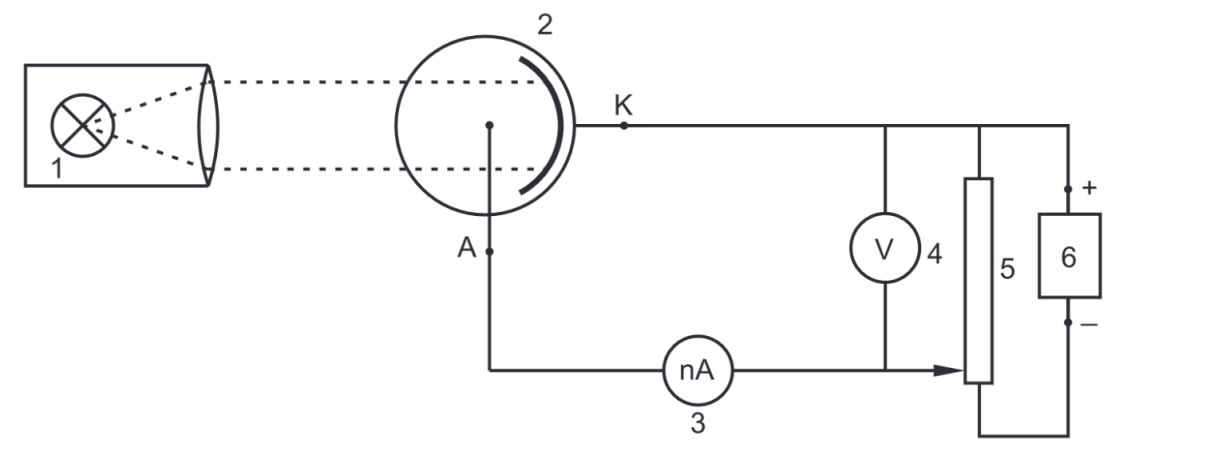
\includegraphics[width=0.9\linewidth]{images/uklad1.png}
	\caption*{Rys. 1 Układ pomiarowy}
\end{figure}



\section*{Przebieg doświadczenia}
\par
Doświadczenie rozpoczęło się od uruchomienia układu pomiarowego.

Dla poszczególnych diod trzykrotnie zmierzyliśmy wartość prądu $I$ powstałego w wyniku emisji elektronów dla napięcia hamującego $U_h = 0$, oraz wartość napięcia odcięcia $U_h$ dla prądu $I = 0$. 

Przedziały $U_h = 0$ do $U_h$ dla którego $I = 0$ zostały podzielone na części dla każdej diody, a następnie dla danych wartości $U_h$ został zmierzony prąd. 

\newpage

\section*{Wyniki pomiarów}
\par
\begin{figure}[H]
	\centering
	\vspace{0pt}
	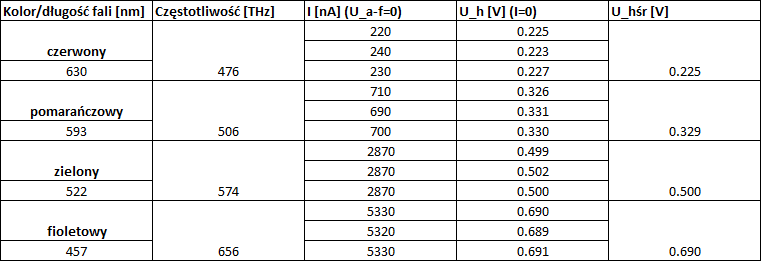
\includegraphics[width=1\linewidth]{images/tabela1.png}
	\caption*{Tabela 1: Pomiary prądu dla $U_h = 0$ i napięcia odcięcia}
\end{figure}

\mbox{}\newline\newline

\begin{figure}[H]
	\centering
	\vspace{0pt}
	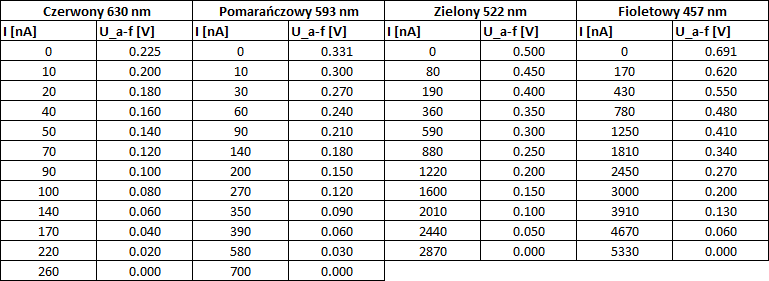
\includegraphics[width=1\linewidth]{images/tabela2.png}
	\caption*{Tabela 2: Pomiary prądu dla ustalonych wartości napięcia}
\end{figure}

\newpage
\section*{Wykresy}
\par
\begin{figure}[H]
	\centering
	\vspace{0pt}
	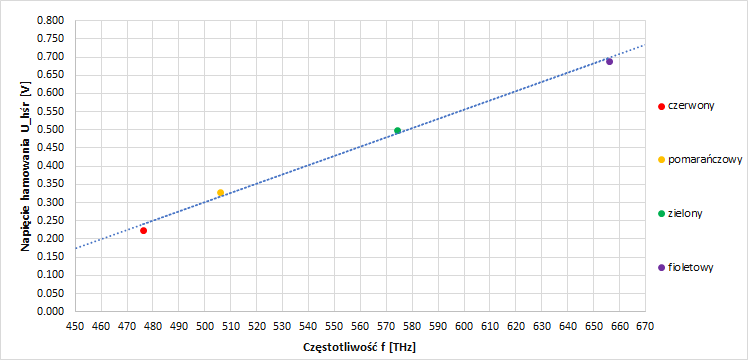
\includegraphics[width=1\linewidth]{images/wykres1.png}
	\caption*{Wykres 1: zależność napięcia hamowania od częstotliwości fal poszczególnych kolorów}
\end{figure}

\mbox{}\newline\newline

\begin{figure}[H]
	\centering
	\vspace{0pt}
	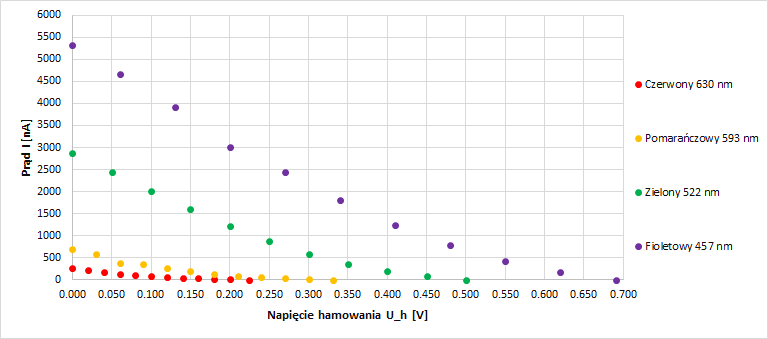
\includegraphics[width=1\linewidth]{images/wykres2.png}
	\caption*{Wykres 2: prąd płynący przez fotokomórkę od napięcia hamowania dla
		poszczególnych kolorów}
\end{figure}

\newpage

\section*{Opracowanie wyników}
\subsection*{Stała Plancka}
\par
Dla danych z Tabeli 1 korzystając z programu \textbf{Excel} przeprowadziliśmy regresję liniową i otrzymaliśmy współczynniki prostej:
\begin{align*}
	a &= 0.0025 \ \frac{\text{V}}{\text{THz}} \ \ u(a) = 0.0001 \ \frac{\text{V}}{\text{THz}} \\
	b &= -0.9699 \ \text{V} \ \quad u(b) = 0.0675 \ \text{V}
\end{align*}

Porównując współczynniki ze wzorem (2):
\begin{gather*}
	U_h = \frac{h}{e}f - \frac{W}{e} , \quad e = 1.6022 \times 10^{-19} \ [C] \\
	\Downarrow \\
	a = \frac{h}{e}, \quad b = - \frac{W}{e} \\
	\Downarrow \\
	h = a \cdot e = 4.0733 \times 10^{-34} \ [J \cdot s]\\
	W = - b \cdot e = 1.5540 \times 10^{-19} \ [J] = 0.9699 \ [eV]
\end{gather*}

\subsection*{Niepewności pomiarowe}
\par Niedokładności przyrządów pomiarowych (woltomierza i amperomierza):
\begin{gather*}
	u(U) =  0.001 \ [\text{V}] \quad u(I) =  10 \ [\text{nA}]
\end{gather*}
\par Niedokładność przy wyznaczaniu stałej Plancka:
\begin{gather*}
	u(a) = u\left(\frac{h}{e}\right) \quad u(b) = u\left(-\frac{W}{e}\right) \\
	u(h) = e \cdot u(a) \quad u(W) = e \cdot u(b) \\\\
	u(h) = 0.1940 \times 10^{-34} \ [J \cdot s] \quad u(W) = 0.0675 \ [eV]
\end{gather*}

\subsection*{Ostatecznie}
\begin{gather*}
	\boxed{h = 4.0733 \times 10^{-34} \pm 0.1940 \times 10^{-34} \ [J \cdot s]}^{\ \ast} \\
	\boxed{W = 0.9699 \pm 0.0675 \ [eV]}
\end{gather*}
	${}^\ast$ Wyznaczona wartość stałej Plancka znacznie odbiega od wartości tabelarycznej ($6.6260 \times 10^{-34} \ [J \cdot s]$) i nie znajduję się w marginesie błędu.

\section*{Wnioski}
\par
Krzywe na wykresach są zgodne z oczekiwaniami, mimo tego nie udało wyznaczyć się stałej Plancka z dużą dokładnością.

Różnica pomiędzy wartością tabelaryczną a wartością otrzymaną może wynikać z:

$\bullet$ Nieznanej wadzie lub niedokładności układu pomiarowego.

$\bullet$ Błędnego przeprowadzania doświadczenia.

Tak duża różnica sugeruje jedną z tych możliwości jako bardziej prawdopodobną niż niedokładność wynikającą z odczytów pomiarów i opracowywania wyników.

\end{document}
